\documentclass[12pt]{article}

\newtheorem{theorem}{Theorem}
\newtheorem{definition}{Definition}
\newtheorem{example}{Example}
\newtheorem{corollary}{Corollary}
\newtheorem{lemma}{Lemma}
\newtheorem{remark}{Remark}
\usepackage{graphicx, hyperref,bm,amsfonts}


\def\R{{\mathbb R}}
\def\X{{\mathcal X}}
\def\Y{{\mathcal Y}}
\def\E{{\mathbb E}}

\textwidth  6.5in \textheight  9.2in \pagestyle{plain}
\parindent=1in
\oddsidemargin 0in
\evensidemargin 1pt
\topmargin -0.61in       %for UNIX


\begin{document}
\small
\begin{center}
\large  \bf STA 243: Homework 2
\end{center}
\vspace{.31in}


 \framebox{\begin{minipage}{0.8\linewidth}
\begin{itemize}
\item Homework due in Canvas: 05/08/2020 at 11:59PM. Please follow the instructions provided in Canvas about homeworks, carefully.
\end{itemize}
 \end{minipage}}

\begin{enumerate}

\item (\textbf{5 Points}) Prove that a differentiable function $f(\theta): \mathbb{R}^d \to \mathbb{R}$ is convex if and only if $$
f(\theta_2) \geq f(\theta_1) + \nabla f(\theta_1)^\top (\theta_2 - \theta_1) 
$$
\textbf{Hint:} Think of 1-dimensional case and extend the intuition to d-dimensional case.

\item (\textbf{20 Points})~The origin of the dataset \texttt{housingprice.csv} we will use in this question is from the Coursera open course Machine Learning Foundations: A Case Study Approach by Prof. Carlos Guestrin and Prof. Emily Fox. Load the training data \texttt{train.data.csv} and testing data \texttt{test.data.csv}. We'll build our regression model on the training data and evaluate the model on the testing data.

\begin{enumerate}
\item Build a linear model on the training data using lm() by regessing the housing price on these variables: \texttt{bedrooms}, \texttt{bathrooms}, \texttt{sqft\_living}, and \texttt{sqft\_lot}. What's the $R^2$ of the model on training data? What's the $R^2$ on testing data?


\item The image below is Bill Gates' house. Load the file \texttt{fancyhouse.csv} to obtain the features of the house. Guess the price of his house using your linear model. Do you think the predicted price is reasonable?
\begin{figure}[!htbp]
\centering
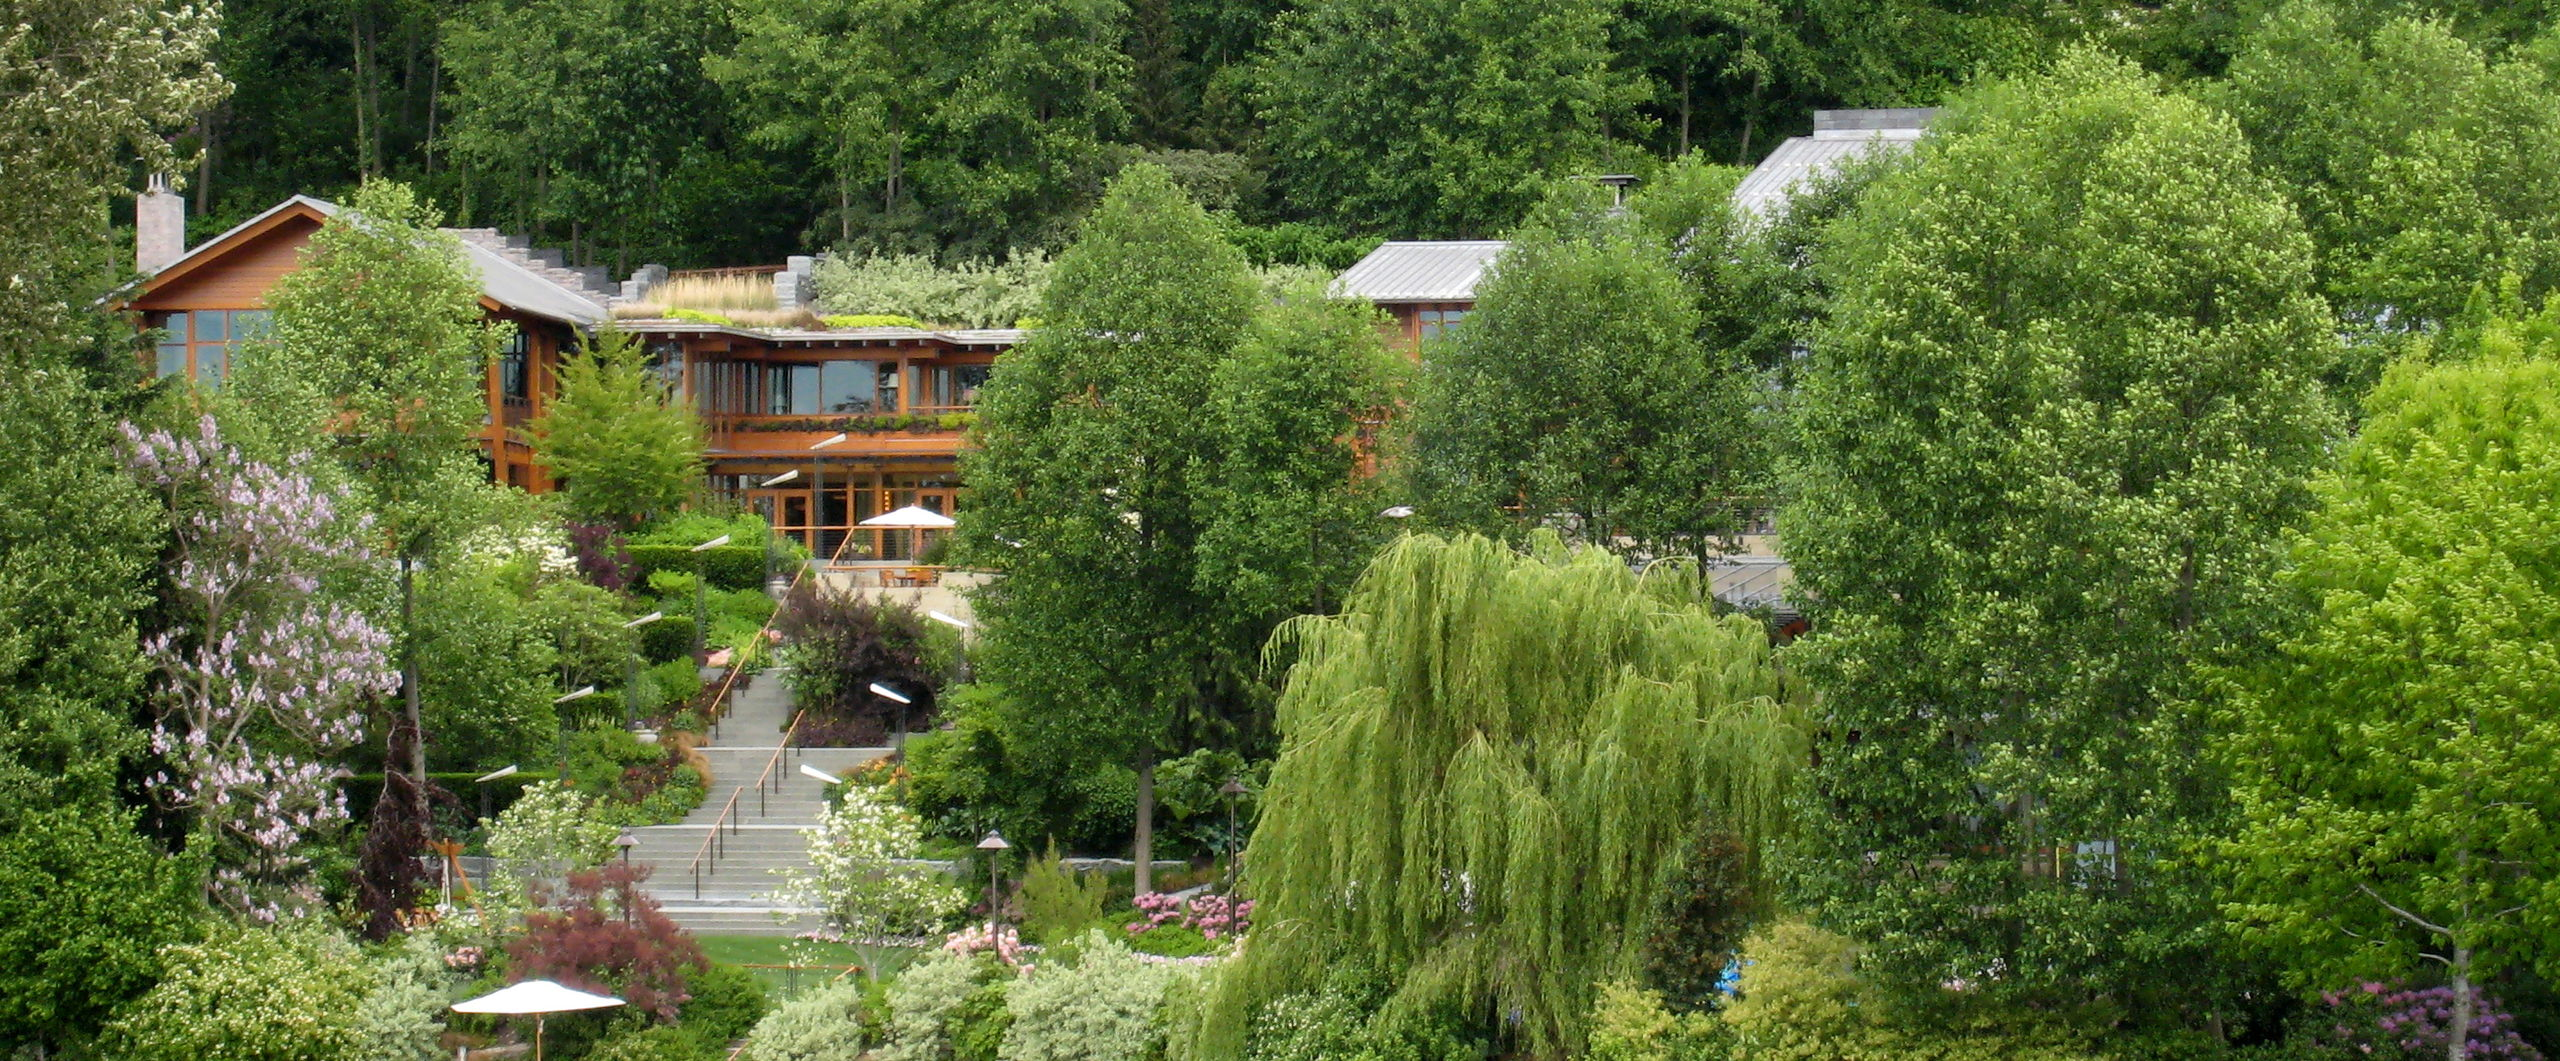
\includegraphics[width = 0.5\textwidth]{./Bill_gates_house.jpg}
\caption{Image from Wikipedia Commons}
\end{figure}

\item Let's continue to improve the linear model we have. Instead of throwing only the raw data into the statistical model, we might want to use our intuition and domain expertise to extract more meaningful features from the raw data. This step is called feature engineering. Using meaningful features in the model is  often crucial for successful data analysis.
 Add another variable by multiplying the number of bedrooms by the number of bathrooms, which describes the combined benefit of having more bedrooms and bathrooms. Add this variable to the linear model we have in Part (a). What's the $R^2$ of the new model on the training data and testing data respectively?

(\textbf{Hint:} You don't have to create a new column in the data frame. Try this trick in \texttt{lm()}:
  \texttt{lm( y $\sim$ x1 + x2 + x1 * x2, data = your.data)})
  
\item Perform all the things above without using the in-built function \texttt{lm()} in R, but by using \texttt{gradient descent algorithm} on the sample-based least-squares objective function, to estimate the OLS regression parameter vector. How does your result compare to the result from previous part ? Note that you have to set the tuning parameter appropriately for this method.

\item Perform all the things above now using \texttt{stochastic gradient descent} (with one sample in each iteration). How does your result compare to the result from previous parts ? Note: while running \texttt{stochastic gradient descent}, you can sample without replacement and when you run out of samples, just start over.  Note that you have to set the tuning parameter appropriately for this method.
\end{enumerate}

\item (\textbf{15 Points}) Prove Fact 6.1.1 in \texttt{OPT.pdf} and solve the recursion to obtain the final result of  Theorem 6.1. (\textbf{Hint:} You can use induction)
\end{enumerate}

\end{document}
